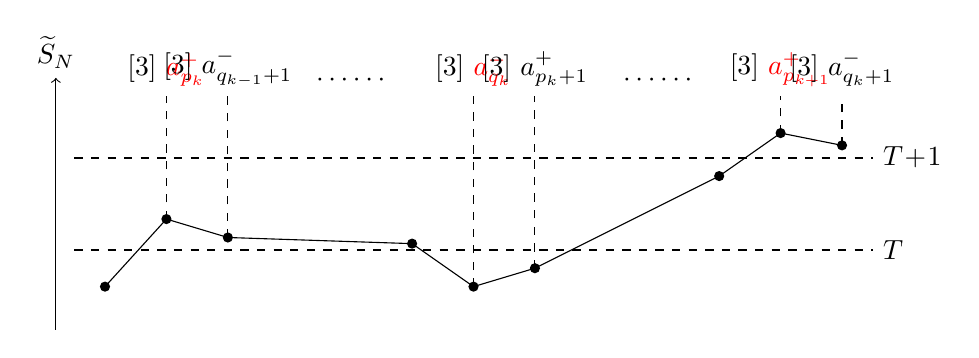
\begin{tikzpicture}[
scale=0.78,
]

\draw[->] (-0.8, -0.3) -- (-0.8, 3.8) node[anchor=south] {$\widetilde{S}_N$};
\draw[dashed, thick] (-0.5, 1.0) -- (12.5, 1.0) node[right] {$T$};
\draw[dashed, thick] (-0.5, 2.5) -- (12.5, 2.5) node[right] {$T\!+\!1$};

% Same x-coordinates as riemann-series-thm.tex: 0,1,2,5,6,7,10,11,12
% Pattern per cycle: exceeds T (peak k) → first neg (still above T) → ... → unlabeled dot
%   (above T) → drops below T (valley k) → first pos (still below T) → ...
%   → unlabeled dot (below T+1) → exceeds T+1 (peak k+1) → first neg (still above T+1)
\draw[thin]
    (0, 0.4) node[fill,circle,inner sep=1.3pt]{}
    \foreach \x/\y in {1/1.5, 2/1.2, 5/1.1, 6/0.4, 7/0.7, 10/2.2, 11/2.9, 12/2.7} {
        -- (\x,\y) node[fill,circle,inner sep=1.3pt]{}
    };

% All dashed lines go from current dot's y up to label area
\draw[dashed, thin] (1,  1.5) -- (1,  3.5) node[anchor=south] {\smaller[3] \color{red} $a_{p_k}^+$};
\draw[dashed, thin] (2,  1.2) -- (2,  3.5) node[anchor=south] {\smaller[3] $a_{q_{k-1}+1}^-$};
\draw[dashed, thin] (6,  0.4) -- (6,  3.5) node[anchor=south] {\smaller[3] \color{red} $a_{q_k}^-$};
\draw[dashed, thin] (7,  0.7) -- (7,  3.5) node[anchor=south] {\smaller[3] $a_{p_k+1}^+$};
\draw[dashed, thin] (11, 2.9) -- (11, 3.5) node[anchor=south] {\smaller[3] \color{red} $a_{p_{k+1}}^+$};
\draw[dashed, thin] (12, 2.7) -- (12, 3.5) node[anchor=south] {\smaller[3] $a_{q_k+1}^-$};

\node[anchor=south] at (4, 3.5) {$\cdots\cdots$};
\node[anchor=south] at (9, 3.5) {$\cdots\cdots$};

\end{tikzpicture}
